\documentclass[../differential_methods.tex]{subfiles}
\begin{document}
\section{Aula 19 - 15 de Junho, 2026}
\subsection{Motivações}
\begin{itemize}
	\item Discretizando a Equação Hiperbólica;
	\item Método Lax-Wendroff.
\end{itemize}
\subsection{Introduzindo Difusão à Advecção}
Utilizamos o método das linhas para discretizar a equação hiperbólica, obtendo
\[
	u_{t}(x_{j}, t) + a \biggl(\frac{u(x_{j+1}, t)-u(x_{j-1}, t)}{2\Delta x}\biggr) + \mathcal{O}(h^{2}) = 0,
\]
mas dessa vez olharemos as condições de contorno periódicas, como se restringíssemos o problema a um círculo ao invés da reta toda.

Consideramos a discretização espacial \(u_{0}(t), u_{1}(t), \dotsc , u_{m}(t), u_{m+1}(t) = u_{0}(t)\); assim, se for necessário aplicar um estêncil centrado, o \(j+1\) do ponto à extrema direita vai ser o mesmo que o ponto logo após o \(0,\) ou seja, o 1 (analogamente para o ponto mais à esquerda).
Como o tempo foi mantido contínuo, temos o sistema de EDOs resultante
\[
	\frac{\mathrm{d}}{\mathrm{d}t}U_{j}(t) + \frac{a}{2\Delta x}(U_{j+1}(t)-U_{j-1}(t)) = 0,
\]
mas é necessário tomar uma decisão se chamaremos os índices de 0 até m ou de 1 até m+1; manteremos este segundo, obtendo, para \(j=1\), o sistema
\[
	\frac{\mathrm{d}}{\mathrm{d}t}U_{1}(t) + \frac{a}{2\Delta x}(U_{2}(t) - U_{m+1}(t)) = 0
\]
e, para \(j=m+1\), o ponto à direita dele ``é o 1'':
\[
	\frac{\mathrm{d}}{\mathrm{d}t}U_{m+1}+\frac{a}{2\Delta x}(U_{1}-U_{m}(t))=0 \Longleftrightarrow \underline{U}'(t) = A \underline{U}(t),\; U_{j}(0) = \eta(x_{j}).
\]

Agora, montamos a forma como isso aparece matricialmente, que será
\[
	\frac{\mathrm{d}}{\mathrm{d}t}\begin{bmatrix}
		U_1(t) \\
		U_2(t) \\
		\vdots \\
		U_{m+1}(t)
	\end{bmatrix} + \frac{a}{2\Delta x}\begin{bmatrix}
		0      & 1      & 0      & \dotsc & 0      & -1     \\
		-1     & 0      & 1      & 0      & \dotsc &        \\
		\vdots & \ddots & \vdots & \vdots & \vdots & \vdots \\
		1      & 0      & \dotsc & 0      & -1     & 0
	\end{bmatrix}\begin{bmatrix}
		U_1(t) \\
		U_2(t) \\
		\vdots \\
		U_{m+1}(t)
	\end{bmatrix}=0
\]
e já de cara dá pra notar que a matriz A é diferente dos casos anteriores pois ela é \textit{antisimétrica}, os elementos acima da diagonal são iguais aos da diagonal inferior, mas com sinais invertidos (\(A^{T} = -A\)), além de que \textbf{todos os seus autovalores são não reais}, com forma
\[
	\lambda_{p} = -i \frac{a}{\Delta x}\sin^{}{(2\pi p \Delta x)}, \quad p=1, 2, \dotsc ,m+1;
\]
assim, por seno variar entre -1 e 1, os autovalores estão todos entre \(-i \frac{a}{\Delta x}\) e \(i \frac{a}{\Delta x}\). Se fossemos resolver por Euler explícito, sabemos onde ficam os seus autovalores de estabilidade, estando no círculo entre -2 e 0, mas todos os autovalores deste método estão no eixo imaginário puro! Logo, o resultado da falta de estabilidade do método de Euler explícito ganhou mais uma explicação.
Qual método que havíamos visto e que foi descartado no método parabólico justamente porque a estabilidade surgia apenas para autovalores imaginários puros? O método do ponto médio:
\[
	\boxed{\underline{U}^{n+2} = \underline{U}^{n} + 2\Delta t \underline{U}F^{n+1}}.
\]
Antes de aplicá-lo, consideremos uma discretização espacial por diferenças progressivas:
\[
	\underline{U}^{n+1} = \underline{U}^{n} + \Delta t A \underline{U}^{n} = \underbrace{(I + \Delta t A)}_{B(\Delta t)}\underline{U}^{n};
\]
então, o método será convergente se conseguirmos \(\Delta t\) tender a 0 mais rápido que \(\Delta x\), por exemplo tomando \(\Delta t = \Delta x^{2}\), caso no qual
\[
	\Vert 1 + \Delta t A \Vert_{2}^{2} = \rho ((I-\Delta tA)(I+\Delta tA)) = \rho (I-\Delta t^{2}A^{2})\leq 1 + \Delta t^{2}\frac{a^{2}}{\Delta x^{2}}=1 + a^{2}\Delta t.
\]
Logo, se \(n\Delta t \leq T\) e \(\Delta t = \Delta x^{2}\), teremos a estabilidade Lax-Richtmeyer
\[
	\Vert (I+\Delta A)^{n} \Vert_{2} \leq (1+a^{2}\Delta t)^{\frac{n}{2}}\leq e^{a^{2}\frac{T}{2}}.
\]
O problema é que essa limitação de \(\Delta t = \Delta x^{2}\) é muito ruim, tornando a análise acima, que parecia muito útil, em inútil.

Agora, utilizando a regra do ponto médio ao PVI, obtemos o chamado \hypertarget{leapfrog_method}{\textbf{método leapfrog}} para a equação hiperbólica:
\[
	\boxed{U_{j}^{n+1} = U_{j}^{n-1} - \frac{a\Delta t}{2\Delta x}(U_{j+1}^{n} - U_{j-1}^{n})},
\]
resultando num método explícito de 3 níveis e de ordem dois tanto no espaço quanto no tempo. Mais ainad, a estabilidade é dada justamente pela condição
\[
	\frac{| a |\Delta t}{\Delta x} \leq 1,
\]
novamente voltando ao número de Courant. Logo, o método leapfrog é um explícito que parece funcionar bem para esse problema.

Retomemos, dessa vez, o método Lax-Friedrichs
\[
	U_{j}^{n+1} = \frac{1}{2}(U_{j-1}^{n}+U_{j+1}^{n}) - \frac{a\Delta t}{2\Delta x}(U_{j+1}^{n}-U_{j-1}^{n})
\]
e somemos \(0 = U_{j}^{n} - \frac{1}{2}2U_{j}^{n}\) em volta do primeiro parêntesis:
\[
	U_{j}^{n+1} = U_{j}^{n} + \frac{1}{2}(U_{j-1}^{n}-2U_{j}^{n}+U_{j+1}^{n}) - \frac{a\Delta t}{2\Delta x}(U_{j+1}^{n}-U_{j-1}^{n}).
\]
Rearranjando, obtemos a expressão
\[
	\frac{U_{j}^{n+1}-U_{j}^{n}}{\Delta t} + a \biggl(\frac{U_{j+1}^{n}-U_{j-1}^{n}}{2\Delta x}\biggr) = \frac{\Delta x^{2}}{2\Delta t}\biggl(\frac{U_{j-1}^{n}-2U_{j}^{n}+U_{j+1}^{n}}{\Delta x^{2}}\biggr),
\]
que ainda é o método Lax-Friedrichs, afinal apenas somamos 0 e multiplicamos 1, mas ele recebeu a discretização de \(u_t\), de \(u_x\) e \(u_{xx}\) à direita da igualdade! Porém, como o método de Lax-Friedrichs é consistente de ordem 2 no espaço e 1 no tempo para a equação do trasporte sem o termo \(\frac{\Delta x^{2}}{2\Delta t}\), estamos essencialmente escrevendo a versão discretizada de uma equação de advecção-difusão
\[
	u_t + a u_x = \varepsilon u_{xx}, \quad \varepsilon = \frac{\Delta x^{2}}{2\Delta t},
\]
tal que, olhando para a matriz de amplificação com o termo \(\varepsilon u_{xx}\),
\[
	A_{\varepsilon } = -\frac{a}{2\Delta x}\begin{bmatrix}
		0      & 1      & 0      & \dotsc &        & -1     \\
		-1     & 0      & 1      & 0      & \dotsc &        \\
		\vdots & \ddots & \vdots & \vdots & \vdots & \vdots \\
		1      & 0      & \dotsc & 0      & -1     & 0
	\end{bmatrix} + \frac{\varepsilon }{\Delta x^{2}}\begin{bmatrix}
		-2     & 1      & 0      & \dotsc &        & 1      \\
		1      & -2     & 1      & 0      & \dotsc &        \\
		       & 1      & -2     & 1      & \dotsc &        \\
		\vdots & \vdots & \vdots & \ddots & \vdots & \vdots \\
		       &        &        & 1      & -2     & 1      \\
		1      & 0      & \dotsc & 0      & -1     & -2
	\end{bmatrix},
\]
os autovalores passam a ter uma parte real:
\[
	\mu_p = -\frac{ia}{\Delta x}\sin^{}{(2\pi p\Delta x)}-\frac{2\varepsilon }{h^{2}}(1-\cos^{}{(2\pi p\Delta x)}),
\]
caindo dentro da região de estabilidade do método de Euler! Os valores \(\Delta t\mu\) estão numa elipse centrada em
\[
	-2\frac{\Delta t\varepsilon }{\Delta x^{2}} = -1,
\]
com semieixos de tamanho \(2\Delta t\varepsilon /\Delta x^{2} = 1\) na direção x e \(a \frac{\Delta t}{\Delta x}\) na direção y, sendo estável quando
\[
	\biggl\vert \frac{a\Delta t}{\Delta x} \biggr\vert\leq 1.
\]
O interessante é que esse tipo de análise não e inédito ao método Lax-Friedrichs, pode ser feito também, por exemplo, no método upwind, entre outros (vide imagem abaixo)
\begin{figure}[H]
	\begin{center}
		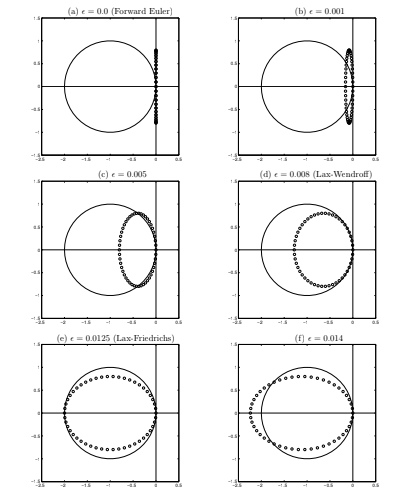
\includegraphics[height=0.7\textheight, width=0.7\textwidth, keepaspectratio]{./Images/kmip_18.png}
	\end{center}
	\caption{alguns exemplos de \(k\mu_p\) para vários valores de \(\varepsilon \) e métodos.}
\end{figure}

O problema de adicionar difusão para conseguir estabilidade é que tem algumas consequências não desejáveis, e o resultando numérico começa a ficar disperso, picos podem sumir e a precisão diminui ao descrever o transporte:
\begin{figure}[H]
	\begin{center}
		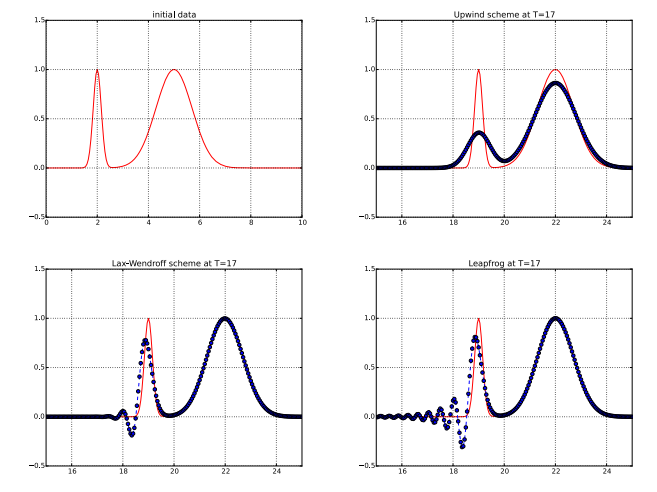
\includegraphics[height=\textheight, width=\textwidth, keepaspectratio]{./Images/numerical_results_19.png}
	\end{center}
	\caption{o pico começa a sumir por conta da dispersão, e até mesmo passa a ter uma oscilação severa da solução.}
\end{figure}

Até agora, estivemos usando diferenças finitas para resolver trasporte, mas elas precisam de expansões em Taylor, por sua vez precisam de derivadas de ordens cada vez maiores e suavidade de graus maiores, mas nem todo transporte usa etapas contínuas! O \textbf{método Lax-Wendroff} é um que existe para problemas descontínuos, mas não é a dedução que vamos fazer aqui porque o foco do curso é justamente a questão das diferenças finitas.
Em sua dedução com diferenças finitas, aplica-se a expansão de Taylor diretamente a \(u_t + au_x = 0\), resultando em
\[
	u(x, t + \Delta t) = u(x, t) + \Delta tu_t (x, t) + \frac{1}{2}\Delta tu_{tt}(x, t) + \dotsc ;
\]
trocando \(u_t = -au_x\) e \(u_{tt}= (-au_x)_t = -a (u_t)_x = a^{2}u_{xx}\), obtemos
\[
	u(x, t+\Delta t) = u(x, t) - \Delta t a u_{x}(x, t) + \frac{1}{2}\Delta t^{2} a^{2}u_{xx}(x, t)+\dotsc
\]
Assim, usando a aproximação central padrão para \(u_x\) e \(u_{xx}\), abandonando termos de ordens superiores, obtemos o \hypertarget{lax_wendroff}{\textbf{método Lax-Wendroff}}
\[
	\boxed{U_{j}^{n+1} = U_{j}^{n} - a \frac{\Delta t}{2\Delta x} (U_{j+1}^{n}-U_{j-1}^{n}) + \frac{a^{2}\Delta t^{2}}{2\Delta x^{2}}(U_{j+1}^{n}-2U_{j}^{n} + U_{j-1}^{n})}
\]

\textbf{\underline{Cuidado}:} apesar do termo da derivada de segunda ordem, a estabilidade do método acima é para a equação \(u_t + au_x = 0\), e ela apenas introduz difusão numérica novamente!
\begin{exr}
	Mostre que o \hyperlink{lax_wendroff}{\textit{método de Lax-Wendroff}} é um método de precisão quadrática no espaço e no tempo, caracterizando o melhor que vimos até o momento para a equação hiperbólica!

	Analise a consistência e estabilidade de todos os métodos da aula de hoje.
\end{exr}
Novamente, podemos examinar a região de estabilidade do Lax-Wendroff, com autovalores
\[
	\Delta t \mu_p = -i \biggl(\frac{a\Delta t}{\Delta x}\biggr)\sin^{}{(p\pi \Delta x)} - \biggl(\frac{a\Delta t}{\Delta x}\biggr)^{2}(1-\cos^{}{(p\pi \Delta x)}),
\]
que resulta novamente no número de Courant menor que 1 como critério de estabilidade.

A ideia de introduzir a difusão numérica aos métodos pode também ser aplicada ao upwind, reescrevendo-o como
\[
	U_{j}^{n+1} = U_{j}^{n} - \frac{a\Delta t}{2\Delta x}(U_{j+1}^{n} - U_{j-1}^{n}) + \frac{a\Delta t}{2\Delta x} (U_{j-1}^{n} - 2 U_{j}^{n} + U_{j+1}^{n}),
\]
que é a discretização de Euler progressivo para \(\underline{U}'(t) = A_{\varepsilon }U(t)\) com \(\varepsilon  = a\Delta x/2\), e é tão parecido com o Lax-Wendroff que dá para repetir a análise de estabilidade; no fim, os três métodos, Lax-Wendroff, upwind e Lax-Friedrichs, podem todos ser vistor como a equação \(u_t + au_x = \varepsilon u_{xx}\), mas com didferentes \(\varepsilon \):
\[
	\varepsilon_{LW} = \frac{a^{2}\Delta t}{2} = \frac{a\Delta x v}{2}, \quad \varepsilon_{UP} = \frac{a\Delta x}{2} \quad\&\quad \varepsilon_{LF} = \frac{\Delta x^{2}}{2\Delta t} = \frac{a\Delta x}{2v},
\]
onde \(v = \frac{a\Delta t}{\Delta x}\). Com isso, obtemos as relações
\[
	\varepsilon_{LW} = v \varepsilon_{UP} \quad\&\quad \varepsilon_{UP} = v\varepsilon_{LF},
\]
de modo que se \(0 < v < 1\), então \(\varepsilon_{LW} < \varepsilon_{UP} < \varepsilon_{LF}\), com os métodos sendo estáveis para qualuqer \(\varepsilon \) entre \(\varepsilon_{LW}\) e \(\varepsilon_{LF}.\)
\end{document}

